\documentclass[a4paper,12pt]{article} % добавить leqno в [] для нумерации слева
\usepackage[a4paper,top=1.3cm,bottom=2cm,left=1.5cm,right=1.5cm,marginparwidth=0.75cm]{geometry}
%%% Работа с русским языком
\usepackage{cmap}					% поиск в PDF
\usepackage[warn]{mathtext} 		% русские буквы в фомулах
\usepackage[T2A]{fontenc}			% кодировка
\usepackage[utf8]{inputenc}			% кодировка исходного текста
\usepackage[english,russian]{babel}	% локализация и переносы
\usepackage{physics}
\usepackage{multirow} %здарова
\usepackage{siunitx}

%%% Нормальное размещение таблиц (писать [H] в окружении таблицы)
\usepackage{float}
\restylefloat{table}

\usepackage{graphicx}

\usepackage{caption}
\usepackage{subcaption}

\usepackage{wrapfig}
\usepackage{tabularx}

\usepackage{hyperref}
\usepackage[rgb]{xcolor}
\hypersetup{
	colorlinks=true,urlcolor=blue
}

%%% Дополнительная работа с математикой
\usepackage{amsmath,amsfonts,amssymb,amsthm,mathtools} % AMS
\usepackage{icomma} % "Умная" запятая: $0,2$ --- число, $0, 2$ --- перечисление

%% Номера формул
%\mathtoolsset{showonlyrefs=true} % Показывать номера только у тех формул, на которые есть \eqref{} в тексте.

%% Шрифты
\usepackage{euscript}	 % Шрифт Евклид
\usepackage{mathrsfs} % Красивый матшрифт
\usepackage{pgfplots}
\pgfplotsset{compat=1.9}

%% Свои команды
\DeclareMathOperator{\sgn}{\mathop{sgn}}

%% Не нумеровать секциии
\setcounter{secnumdepth}{0}

%% Перенос знаков в формулах (по Львовскому)
\newcommand*{\hm}[1]{#1\nobreak\discretionary{}
	{\hbox{$\mathsurround=0pt #1$}}{}}

\date{\today}

\begin{document}

\begin{titlepage}
	\begin{center}
		{\large МОСКОВСКИЙ ФИЗИКО-ТЕХНИЧЕСКИЙ ИНСТИТУТ (НАЦИОНАЛЬНЫЙ ИССЛЕДОВАТЕЛЬСКИЙ УНИВЕРСИТЕТ)}
	\end{center}
	\begin{center}
		{\large Физтех-школа прикладной математики и информатики}
	\end{center}
	
	
	\vspace{4.5cm}
	{\huge
		\begin{center}
			{\bf Отчёт о выполнении лабораторной работы 5.5}\\
			Компьютерная сцинтилляционная $\gamma$-спектрометрия
		\end{center}
	}
	\vspace{1cm}
	\begin{center}
		{\large Соболевский Федор Александрович \\
  Старокожко Иван Георгиевич
			\vspace{0.2cm}
			Б05-111}
	\end{center}
	\vspace{8cm}
	\begin{center}
		  Декабрь 2023
	\end{center}
\end{titlepage}

\section{Теоретические положения}
	
Основная задача спектрометрических измерений заключается в определении энергии, интенсивности дискретных гамма-линий от различных гамма-источников и их идентификации.
	
Основными процессами взаимодействия гамма-излучения с веществом являются фотоэффект, эффект Комптона и образование электрон-позитронных пар. Каждый из этих процессов вносит свой вклад в образование наблюдаемого спектра. Образующиеся при этих процессах электроны испытывают большое количество неупругих соударений с молекулами и атомами среды. Неупругие соударения могут сопровождаться как ионизацией, так и возбуждением молекул или атомов среды. В промежуточных же стадиях (при переходах возбужденных молекул или атомов в основное состояние, при рекомбинации электрических зарядов и т.п.) в веществе возникают кванты света различных длин волн, присущих данному веществу.
	
При \textbf{фотоэффекте} кинетическая энергия электрона $ T_e = E_\gamma - I_i $, где $ I_i $ --- энергия ионизации $ i $-той оболочки атома. Фотоэффект особенно существенен для тяжелых веществ, где он идет с заметной вероятностью даже при высоких энергиях гамма-квантов. В легких веществах фотоэффект становится заметен лишь при относительно небольших энергиях гамма-квантов. Наряду с фотоэффектом, при котором вся энергия гамма-кванта передается атомному электрону, взаимодействие гамма-излучения со средой может приводить к его рассеянию, т.е. отклонению от первоначального направления распространения на некоторый угол.
	
При \textbf{эффекте Компотна} происходит упругое рассеяние фотона на свободном электроне, сопровождающееся изменением длины волны фотона (реально этот процесс происходит на слабо связанных с атомом внешних электронах). Максимальная энергия образующихся комптоновских электронов соответствует рассеянию гамма-квантов на $ 2\pi $ и равна
	
\begin{equation}\label{E_compton}
    E_{max} = \dfrac{\hbar \omega}{1 + \dfrac{m_ec^2}{2\hbar\omega}}
\end{equation}
	
При достаточно высокой энергии гамма-кванта наряду с фотоэффектом и эффектом Комптона может происходить третий вид взаимодействия гамма-квантов с веществом – \textbf{образование электрон-позитронных пар}. При этом если процесс образования пары идет в кулоновском поле ядра или протона, то энергия образующегося ядра отдачи оказывается весьма малой, так что пороговая энергия гамма-кванта, необходимая для образования пары, практически совпадает с удвоенной энергией покоя электрона $ E_0 = 2m_ec^2 =1,022  $МэВ.
	
Появившийся в результате процесса образования пар электрон теряет свою энергию на ионизацию среды. Таким образом, вся энергия электрона остается в детекторе. Позитрон будет двигаться до тех пор, пока практически не остановится, а затем аннигилирует с электроном среды, в результате чего появятся два гамма-кванта. Т.е., кинетическая энергия позитрона также останется в детекторе. Далее возможны три варианта развития событий:
	
а) оба родившихся гамма-кванта не вылетают из детектора, и тогда вся энергия первичного гамма-кванта останется в детекторе, а в спектре появится пик с $ E = E_\gamma $;
	
б) один из родившихся гамма-квантов покидает детектор, и в спектре появляется пик, соответствующий энергии $  E = E_\gamma - E_0 $, где $ E_0 = m_ec^2 = $ 511 кэВ;
	
в) оба родившихся гамма-кванта покидают детектор, и в спектре появляется пик, соответствующий энергии $  E = E_\gamma - 2E_0 $, где $ 2E_0 = 2m_ec^2 = $ 1022 кэВ;
	
Таким образом, любой спектр, получаемый с помощью гамма-спектрометра, описывается несколькими компонентами, каждая из которых связана с определенным физическим процессом. Как описано выше, основными физическими процессами взаимодействия гамма-квантов с веществом являются фотоэффект, эффект Комптона и образование электрон-позитронных пар, и каждый из них вносит свой вклад в образование спектра. Помимо этих процессов, добавляются экспонента, связанная с наличием фона, пик характеристического излучения, возникающий при взаимодействии гамма-квантов с окружающим веществом, а также пик обратного рассеяния, образующийся при энергии квантов $ E_\gamma \gg mc^22/2 $ в результате рассеяния гамма-квантов на большие углы на материалах конструктивных элементов детектора и защиты. Положение пика обратного рассеяния определяется по формуле ($ E $ --- энергия фотопика):
	
\begin{equation}\label{Eobr}
    E_\text{обр} = \dfrac{E}{1 + \dfrac{2E}{mc^2}}
\end{equation}

\section{Экспериментальная установка}
\begin{figure}
    \centering
    \includegraphics[width=0.5\textwidth]{setup.png}
    \caption{Принципиальная блок-схема спектрометра. (1 – сцинтиллятор, 2 – ФЭУ, 3 – предусилитель импульсов, 4 – высоковольтный блок питания для ФЭУ, 5 – блок преобразования аналоговых импульсов с ФЭУ в цифровой код (АЦП), 6 – компьютер для сбора данных, их обработки и хранения).}
    \label{fig:setup}
\end{figure}

Энергетическим разрешением спектрометра называется величина	
\begin{equation}\label{Ri = dE/E}
    R_i = \dfrac{\Delta E_i}{E_i}
\end{equation}
т.е. отношение ширины пика полного поглощения (измеренной на полувысоте) к регистрируемой энергии пика поглощения. Это значение $ E_i \propto \overline{n_i} $ --- числу частиц на выходе ФЭУ. При этом  $ \Delta E_i \propto \overline{\Delta n_i} = \sqrt{\overline{n_i}} $ --- ширина пика пропорциональна среднеквадратичной флуктуации, которая равна корню из числа частиц. Таким образом, наша формула \eqref{Ri = dE/E} примет вид
	
\begin{equation}\label{Ri = c/E}
    R_i = \dfrac{\mathrm{const}}{\sqrt{E_i}}
\end{equation}

Принципиальная блок-схема гамма-спектрометра, изучаемого в данной
работе, показана на рис. \ref{fig:setup}. ФЭУ со сцинтиллятором и блоком питания установлены на отдельной подставке. В нашей работе на разных установках (стендах) в качестве сцинтиллятора используются кристаллы NaI(Tl).

\newpage
\section{Результаты измерений и обработка экспериментальных данных}

Перед началом работы с образцами был измерен фон, присутствующий во время каждого эксперимента. Спектр фонового излучения представлен на рис.~\ref{fig:background}. В дальнейшем мы будем из полученных для образцов результатов вычитать этот фон.
\begin{figure}[h]
    \centering
    \includegraphics[width=0.50\textwidth]{background.png}
    \caption{Спектр фонового излучения}
    \label{fig:background}
\end{figure}


Были измерены спектры для следующих веществ: $^6^0$Co, $^2^2$Na, $^1^3^7$Cs, $^1^5^2$Eu и $^2^4^1$Am. Графики представлены на рис.~\ref{fig:CoNa}, \ref{fig:Cs} и \ref{fig:EuAm}. По этим графикам определим пики, соотвествующие фотопикам $^6^0$Co, $^2^2$Na и $^1^3^7$Cs (см. таблицу~\ref{tab:peaks}) и построим по этим данным калибровочный график $E = E(N)$ (см. рис.~\ref{fig:calibr}). Полученная методом наименьших квадратов зависимость и погрешности коэффициентов:
\begin{equation}\label{NtoE}
    E = aN + b,\quad\text{где }a = (0,767\pm0,003)\text{ кэВ, }b = (-47,9\pm3,8)\text{ кэВ.}
\end{equation}
\begin{table}[h]
    \centering
    \begin{tabular}{|c|c|c|c|c|c|} \hline
         & \multicolumn{2}{|c|}{$^6^0$Co} & \multicolumn{2}{|c|}{$^2^2$Na} & $^1^3^7$Cs \\ \hline
        Энергия пика $E$, МэВ & 1,173 & 1,332 & 0,511 & 1,274 & 0,662 \\ \hline
        Номер линии $N$  & 1592 & 1804 & 729 & 1720 & 926 \\ \hline
    \end{tabular}
    \caption{Энергии пиков, используемые для калибровки}
    \label{tab:peaks}
\end{table}
\begin{figure}[h]
    \centering
    \includegraphics[width=0.6\textwidth]{calibr.png}
    \caption{Калибровочный график зависимости энергии квантов от номера канала}
    \label{fig:calibr}
\end{figure}

Используя калибровочную зависимость, пересчитаем данные о положении и ширине пиков для всех спектров и вычислим для каждого значение разрешающей способности $R$ по формуле \eqref{Ri = dE/E}.
\begin{table}[h]
    \centering
    \begin{tabular}{|c|c|c|c|c|c|c|c|c|c|} \hline
         & \multicolumn{2}{|c|}{$^6^0$Co} & \multicolumn{2}{c|}{$^2^2$Na} & $^1^3^7$Cs & \multicolumn{3}{c|}{$^1^5^2$Eu} & $^2^4^1$Am \\ \hline
        Центр пика $N$ & 1592 & 1804 & 729 & 1720 & 926 & 114 & 228 & 512 & 144 \\ \hline
        Полуширина пика $\Delta N$ & 81 & 72 & 54 & 75 & 60 & 17 & 16 & 37 & 13 \\ \hline
        Энергия пика $E$, МэВ & 1,173 & 1,332 & 0,511 & 1,274 & 0,662 & 0,395 & 0,127 & 0,345 & 0,063 \\ \hline
        Полуширина $\Delta E$, МэВ & 0,062 & 0,055 & 0,041 & 0,057 & 0,046 & 0,013 & 0,012 & 0,028 & 0,010 \\ \hline
        Разрешение $R$ & 0,053 & 0,041 & 0,081 & 0,045 & 0,069 & 0,330 & 0,097 & 0,082 & 0,159 \\ \hline
    \end{tabular}
    \caption{Параметры пиков и соответствующие им значения разрешения спектрометра}
    \label{tab:peak_resolution}
\end{table}

График зависимости $R^2 = f(1/E)$ приведён на рис.~\ref{fig:Rsquare}. В целом зависимость довольно хорошо аппроксимируется линейной с одним выбросом и коэффициентом $k = (239 \pm 20)$ МэВ.

\begin{figure}[h]
    \centering
    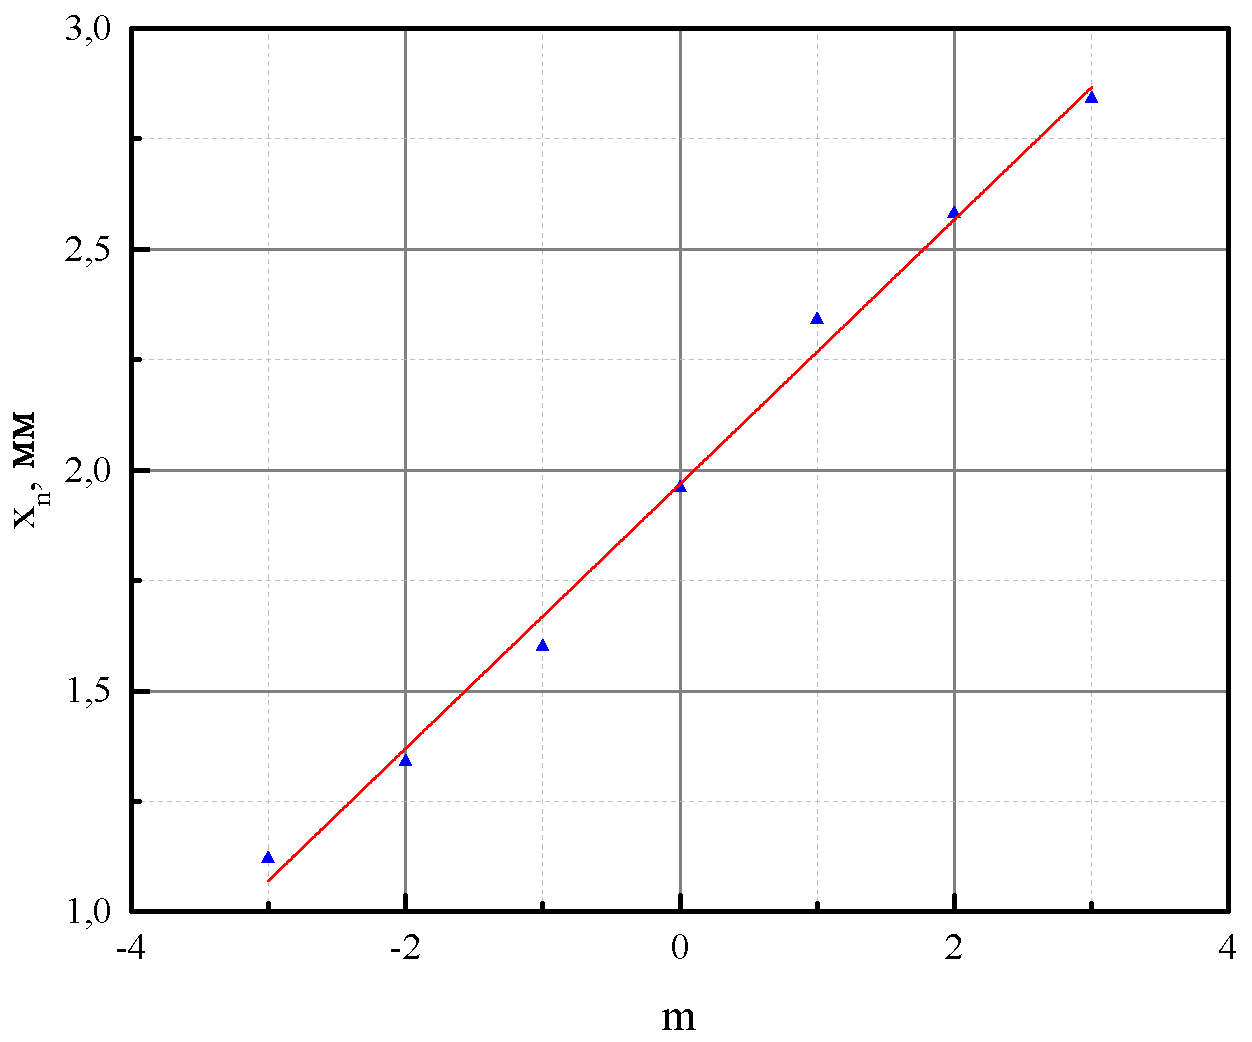
\includegraphics[width=0.6\textwidth]{graph2.png}
    \caption{График зависимости R^2(1/E)}
    \label{fig:Rsquare}
\end{figure}

\section{Вывод}
Нам удалось с помощью сцинтилляционного спектрометра исследовать спектры нескольких слабо радиоактивных веществ. Полученные графики хорошо соотносятся с приведёнными в пособии, а положения пиков дают практически идеальную калибровочную прямую для дальнейших измерений. При установлении зависимости разрешающей способности от энергии $\gamma$ квантов возникли погрешности из-за значений, близких к нулю, которые вносят большую ошибку при расчетах.

\newpage
\section{Приложение}

\begin{figure}[h]
    \centering
    \includegraphics[width=\textwidth]{Na22Co60.png}
    \caption{Спектр излучения изотопов $^6^0$Co, $^2^2$Na}
    \label{fig:CoNa}
\end{figure}
\begin{figure}[h]
    \centering
    \includegraphics[width=0.50\textwidth]{Cs137.png}
    \caption{Спектр излучения изотопа $^1^3^7$Cs} 
    \label{fig:Cs}
\end{figure}
\begin{figure}[h]
    \centering
    \includegraphics[width=\textwidth]{Eu152Am241.png}
    \caption{Спектр излучения изотопов $^1^5^2$Eu и $^2^4^1$Am}
    \label{fig:EuAm}
\end{figure}

\end{document}
